\documentclass[12pt]{article}
\usepackage{blindtext}
\usepackage{graphicx}
\usepackage{subcaption}
\usepackage{float}

\graphicspath{{./images/}}

\title{Finding the most efficient braking position for any bike\\
	\large International Baccalaureate Extended Essay}
\author{Igor Krzywda}

\begin{document}
\maketitle

\section{Introduction}
\subsection{Context}
Braking is the most important safety feature on a bicycle, however when misused braking can be the cause of the
most severe crashes one can have on a bicycle. Many of such crashes are caused by the lack of understanding of
mechanics of braking a bicycle. There are countless tutorials as how to brake properly on a bicycle, but most of
them are based on empirical experience of more proffesional riders. Such advice falls in line with physical 
analysis, but is mostly biased by many factors spanning from the type of cycling the tutorial is based on to 
the attitude towards crashing of the presenter. There is clearly a void in giving an objective advice on safety 
on a bicycle that can be a base to domain-specific guides.

\subsection{Scope of research}
This essay will be exploring the placement of centre of mass for maximum braking while maintaining safety. 
The analysis will be split into two parts-a theoretical one involving building an universal model for finding 
best braking setup and a practical one, which will serve as a validation of the theoretical model using sensor
data.

\subsection{The goal of the research}
The goal of the research is to create an universal model for finding the best braking position in terms of
centre of mass on any bicycle. Such model will serve as a basis for explaining why it is important to find 
a bike fitting its rider and giving the reader an idea of where the limits of his equipment are without 
finding about it by crashing.

\section{Theoretical analysis of braking a bicycle}
\subsection{Rules and assumptions for the analysis}
Assumptions about bicycle and rider:
\begin{itemize}
\item{the rider is a stiff body}
\item{there is no dissipation of force}
\end{itemize}
Safe braking in the analysis is defined by two factors:
\begin{itemize}
\item{rear wheel makes contact with the surface at all times}
\item{no wheel is skidding while braking}
\end{itemize}
Neglected factors\footnote[1]{these factors play more significant role in reality than they do in theoretical
considerations}:
\begin{itemize}
\item{decrease in braking power due to heat and brake pad residue}
\item{dynamic change in frame geometry due to amortisation and tire compression}
\item{air drag}
\item{rolling resistance}
\end{itemize}
\newpage

\subsection{Theoretical model of bicycle and cyclist}
The model of bike and a rider for this analysis is two dimensional, because no lateral forces are taken in 
consideration. The cases for safe braking are checked with the state of wheels, hence the focal point of the 
analysis will be forces excerted on axles, so the whole frame of the bike can be reduced to a single beam 
spanning from axle to axle. The rider is reduced to net centre of mass of bike and cyclist, which is connected
perpendicularly to the virtual beam. Figure~\ref{bike_diagram_1} shows the simplification of the model.
\begin{figure}[h]
\caption{}
\centering
\begin{subfigure}[b]{0.4\linewidth}
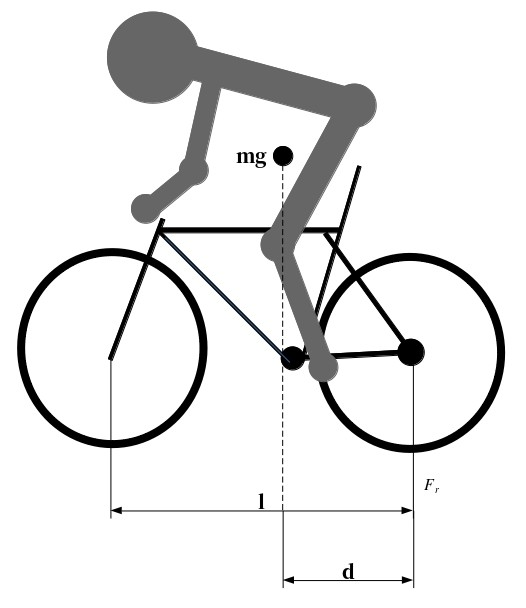
\includegraphics[width=\linewidth]{bike_static_model_bike}%
\label{fig:bike_diagram}
\caption{}
\end{subfigure}
\begin{subfigure}[b]{0.4\linewidth}
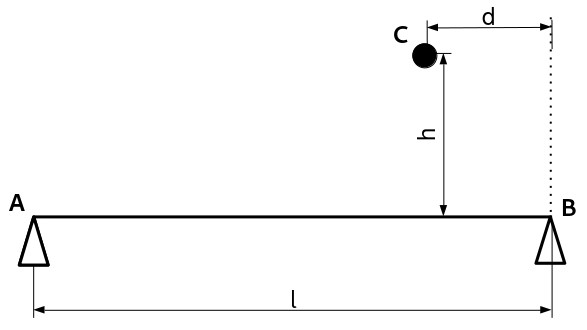
\includegraphics[width=\linewidth]{bike_static_model_simplified}
\caption{}%
\label{fig:beam_diagram}
\end{subfigure}%
\label{fig:theoretical_models}
\end{figure}

\newpage

\subsection{Force distribution on the axles}
The force distribution on the axles is the most important part of the analysis, as it gives us data to 
determine the deceleration and whether or not the conditions for safe braking are maintained.
\begin{figure}[H]
\caption{diagram for calculation of forces on axles}
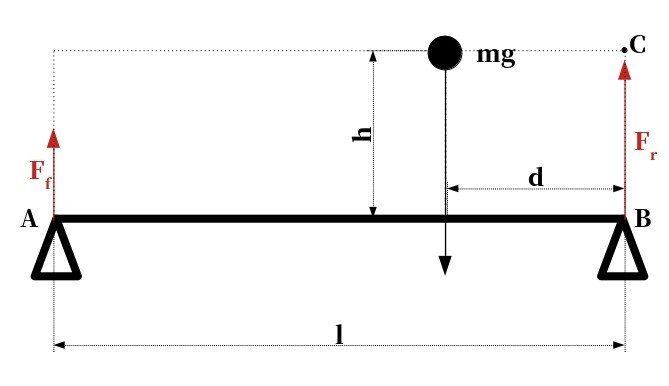
\includegraphics[width=\linewidth]{static_forces_simplified}%
\label{fig:static_diagram}
\end{figure}

\subsubsection{Cyclist static or moving at constant speed}
First let us consider the case of the cyclist being stationary or moving at a constant speed. In order to 
calculate the forces on each axle, we need to consider moments of force applied to the frame, which will be
our moment arm (fig.~\ref{fig:static_diagram}). When a cyclist is on the bike, the point on the frame, where
the force is being excerted is right below his centre of mass. In order to calculate the either of the forces 
on the axles, we need to equate internal torques to either point A or B in fig.~\ref{fig:static_diagram}: 
\emph{$F_f l = mg \cdot d, F_f = \frac{mg \cdot d}{l}$}. Because the net force of the system is the weight
of the rider with the bike, the force on the other axle is \emph{$F_r = mg - F_f$}. \\
\begin{figure}[H]
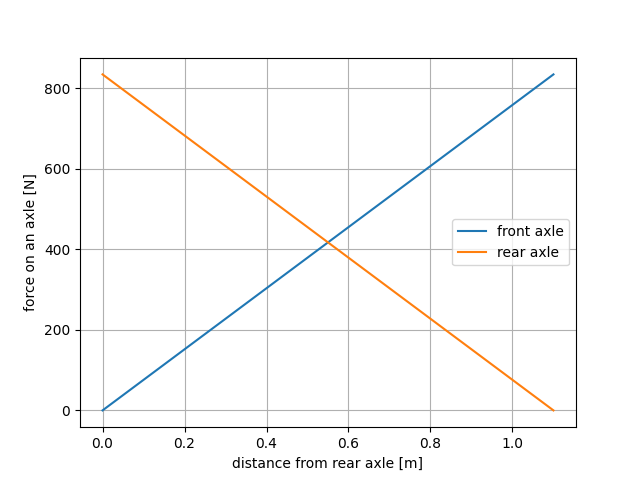
\includegraphics[width=\linewidth]{axles_static_graph}%
\label{fig:static_graph}
\end{figure}
When we plot these equations as functions of the distance, fig.~\ref{fig:static_graph}\footnote[1]{graph is 
generated with parameters from the experiment}. The load on the front axle is a linear function with 
coefficient of $\frac{mg}{l}$, which means that the heavier the rider and bike, the steeper the graph.
Same effect would have been making the bike shorter. The force on the rear axle is the inverse of front one.

\subsubsection{Cyclist decelerating}
For this moment we will consider cyclist just decelerating neglecting what is happening to wheels, focusing
our attention on axles just like in section above. When decelerating, aside from forces caused by the weight, 
we also need to consider force coming from deceleration of the body. From second Newton's law we know that 
$F = ma$, however we are considering our problem in terms of torque, so we need to find the lever arm this
force is acting upon. As mentioned above we are assuming that bicycle and the rider are one rigid body. 
Having assume that, we can say that the centre of mass of bike and rider is connected with a virtual lever
connected at 90 degrees to our main moment arm, which is bike frame (fig.~\ref{fig:theoretical_models}
\subref{fig:beam_diagram}). Just like before, we need to equate the moments, but in this case, we need to 
equate them to point C, as we need to include vertical lever (fig.~\ref{fig:static_diagram}): 
$F_f * l = mg * d + ma * h, F_f = frac{mg * d + ma * h}{l}$. And just like in previous example, 
the force in the rear is: $F_r = mg - F_f$.In this case, however, it is possible for forces to be 
negative (fig~\ref{fig:dynamic_graph}).
\begin{figure}[H]
\caption{}
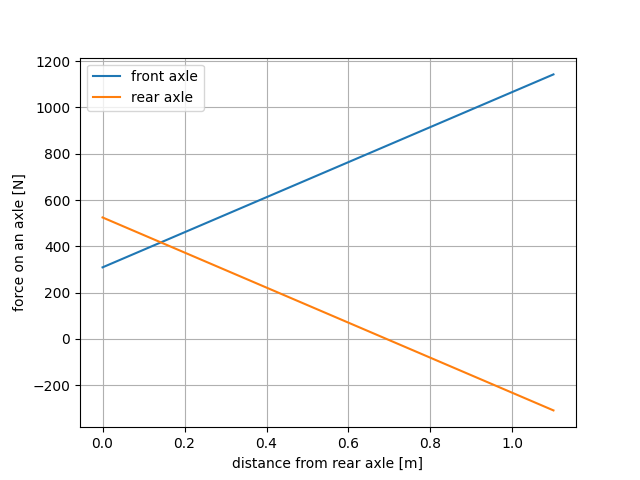
\includegraphics[width=\linewidth]{axles_dynamic_graph}%
\label{fig:dynamic_graph}
\end{figure}

\section{Physical explanation of safe braking}
\subsection{Maintaining rolling of wheels while braking}
\begin{figure}[H]
\caption{}
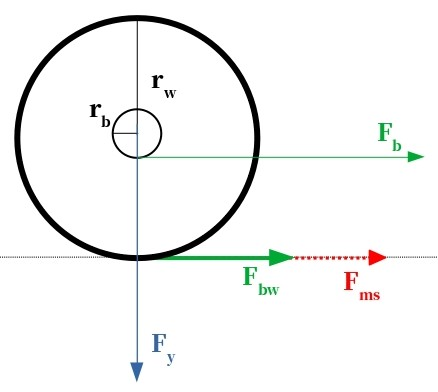
\includegraphics[width=0.75\textwidth]{wheel_braking_forces}%
\label{fig:wheel_diagram_1}
\end{figure}
The limiting factor for braking without skidding is the maximum frictional force between the tire and the 
surface, which is calculated by:
\begin{equation}
\centering%
\label{eq:F_ms}
F_{ms} = F_y \cdot \mu
\end{equation}
When the braking force exceeds the maximum frictional force, the wheel locks up. In order to compare braking 
force with maximum friction, we need to find the braking vector with the same origin as the friction. We do 
that by equating torques to that point like so:
\begin{equation}
\centering%
\label{eq:F_bw}
F_b \cdot r_b = F_{bw} \cdot r_w
\end{equation}
In figure~\ref{fig:wheel_diagram_1} we are analysing wheel with a disk brake, the other type of brake is 
V-brake, which clamps down on the rim with rubber pads, which means that the vector $F_b$ in that case would 
have its origin on the rim. Because of such variations, we will be refering to the braking force in reference 
to the tire-surface contact point rather than the force between brake pad and braking surface.

\subsection{Keeping rear wheel from lifing off}
\end{document}
